%! Suppress = EnDash
\chapter[Setting Up]{Setting Up The Development Environment}\label{ch:setting-up}
\section{Introduction}\label{sec:setting-up-introduction}
To start developing software for the lab, we are going to need different programs. The process of installing programs is different depending on the operating system. It is almost impossible to keep an up-to-date detailed instruction set for every possible version of each program and every possible hardware configuration. The steps below are general and should not present issues. When in doubt, it is always best to check the instructions that the developers of the different packages provide, or ask in the forums.

\section{Python or Anaconda}\label{sec:python-or-anaconda}
If you are already familiar with Python, you probably have encountered that different distributions are worth discussing. Python, in itself, is a text document that specifies what to expect when certain commands are encountered, giving much freedom to develop different implementations of those specifications, each one with different advantages. The \emph{official} distribution is available at python.org and it is the distribution maintained by the Python Software Foundation. In the following sections, we discuss step by step how to install it. This distribution is also referred to as CPython because it is written in the programming language \textbf{C}. The official distribution follows the specification of Python to the letter and therefore is the one that comes bundled with Linux and Mac computers. Newer versions of Windows will start shipping with the official Python distribution.

However, the base implementation of Python left some room for improvement in certain areas. Some developers started to release optimized Python distributions tailored for specific tasks. For example, Intel released a specially designed version of Python to support multi-core architectures, and that leverages specific, low-level libraries developed by themselves. There are other versions of Python, such as Pypy, Jython, Iron Python, and others. Each one has its own merits and drawbacks. Some can run much faster in some contexts but at the expense of limiting the number of things that you can do. Between this wealth of options, there is one that is very popular amongst scientists and everyone doing numeric computations called \emph{Anaconda}, and that we cover in this book.

To expand Python, we can use external packages that can be developed and made publicly available by anyone. Some time ago, the python package manager was limited; it allowed us to install only more straightforward packages. There was a clear need to have a tool that allowed to install more complex packages, including libraries not written in Python. Most numerical programs rely on libraries written in lower-level programming languages such as Fortran or C, and those libraries are not always easy to install in all operating systems, nor to keep track of their dependencies and versions. Anaconda was born to address these issues and is still thriving nowadays. Anaconda is a distribution of Python that comes with \emph{batteries included} for scientists. It includes many Python libraries by default and also supporting programs. It also includes a potent package manager that allows us to install highly optimized libraries for different environments, regardless of whether we are using Windows, Linux, or Mac.

The first edition of this book included instructions for using exclusively plain Python because Anaconda is overkill for the purposes we are covering. However, it is common for researchers to have Anaconda installed on their computers. Therefore, we decided to show how to work with it. If you are starting from scratch, we highly encourage you to start with Anaconda, because it makes your life as a scientist easier. However, if you are using a more limited computer or your installation options are limited, you can use plain Python. For this book, it is simple to install all the libraries required with either system.

\section{Installing Anaconda}\label{sec:installing-anaconda}
To install Anaconda, you just need to head to the official website: anaconda.com. Go to the download section and select the installer of the newest version of Python. It usually auto-detects your operating system and offers you either a graphical installation (recommended) or a command-line one. If you are on Linux, you have to be careful whether you want the Anaconda Python to become your default Python installation. Typically, there won't be any issues; you just need to be aware of the fact that other programs that rely on Python use the Anaconda version and not the stock version.

\tipsInfo{Note}{Similar to the different distributions of Python, Anaconda also comes in two primary flavors: Anaconda and Miniconda. The main difference is that the latter bundles fewer programs and therefore is lighter to download. Unless you are very low in space on your computer or you have particular requirements, we strongly recommend downloading Anaconda.}

\subsection{Using Anaconda}\label{subsec:using-anaconda}
Even though Anaconda comes with a graphical interface to installing packages, throughout the book, we favor the command line because it is easier to transmit ideas with words. If you are on Windows, you need to start a program called \emph{Anaconda Prompt}, such as we show in the image below:

\begin{center}
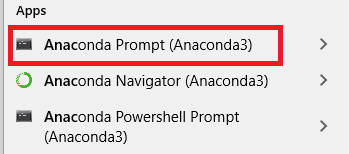
\includegraphics[width=.5\textwidth]{images/Chapter_02/AnacondaPrompt_Menu.png}
\end{center}

If you are on Linux, you only need to open a terminal. On Ubuntu, you can do this by pressing Ctrl+Alt+T. What is important to note is that when you trigger Anaconda, you see that your command line has a \mintinline{bash}{(base)} prepending it. This is the best indication to know you are running on Anaconda installation, as you can see in the image below:

\begin{center}
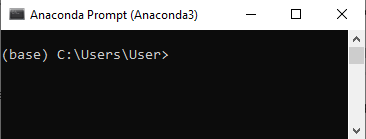
\includegraphics[width=.5\textwidth]{images/Chapter_02/AnacondaPrompt.png}
\end{center}

You can run the following command to see all the installed packages:

\begin{minted}{bash}
conda list
\end{minted}

The output depends on what you have installed, and if you have already used Anaconda in the past. In any case, you see that at the beginning it tells you where the Anaconda installation is, and then you have 4 columns: Name, Version, Build, and Channel, something like this:

\begin{minted}{bash}
# packages in environment at /opt/anaconda3:
#
# Name                    Version                   Build  Channel
matplotlib                3.1.3                    py37_0
numpy                     1.18.1           py37h4f9e942_0
pyyaml                    5.3              py37h7b6447c_0
yaml                      0.1.7                had09818_2
\end{minted}

I have just selected some of the packages as an example, but the output should be much longer. One of the good things about Anaconda is that it keeps track of not only the package and its version but also the build. The difference is that you may be using Anaconda on a computer with an Intel processor, or a Raspberry Pi with an ARM processor. In both cases, the version of, let's say, numpy may be the same, but they were compiled differently. Also, you could be using the same version of numpy but with a different version of Python, hence the \py{py37} that appears in the build numbers, allowing you to keep full track of what you are doing at every moment.

The last two lines show you a package called \py{pyyaml} that depends on a library called \py{yaml}, and that we use later. With Anaconda, you can keep track of both separately, the Python package and the lower-level library that this package uses. If you come from Linux, this is not a great surprise, since this is what package managers do. If you come from Windows, however, this is something incredibly handy.

Let's say we would like to install a package that is not yet available. A package that we use later in the book is called \py{PySerial}. Installing it becomes as easy as running the following command:

\begin{minted}{bash}
conda install pyserial
\end{minted}

It outputs some information, such as the version and the build, and it asks us if we want to install it. We can select 'yes', and it proceeds. If we list the installed packages again, you notice that PySerial is on it.

But this is not all Anaconda allows us to. We can also separate environments based on your projects.

\subsection{Conda Environments}\label{subsec:conda-environments}
A conda environment is, in practical matters, a folder where all the packages that we need to run code are located, including also the underlying libraries. The environments are isolated from each other; therefore, if you update or delete a package on one, it does not affect the others. When you are working on different projects, perhaps one of them needs a specific version of a library, and you don't want to ruin the other projects. To create a new environment, you need to run the following command (change \py{myenv} by any name you want):

\begin{minted}{bash}
 conda create --name myenv
\end{minted}

And then we activate it:

\begin{minted}{bash}
 conda activate myenv
\end{minted}

If now you list the installed packages you will see there is nothing there:

\begin{minted}{bash}
conda list
# packages in environment at /opt/anaconda3/envs/myenv:
#
# Name                    Version                   Build  Channel
\end{minted}

Now is time to install the packages we want, starting with Python itself:

\begin{minted}{bash}
 conda install python=3.7
\end{minted}

\infoInfo{Python Versions}{The \py{3.7} that we added after Python specifies which version of Python we want to use. If you don't specify it, Anaconda installs the newest version, which at the time of writing is \py{3.8}. When Python updates, some libraries may not work correctly, or may not be available yet for that specific version. When selecting the Python version, be sure all your libraries are available.}

After installing Python, you can start it by running:

\begin{minted}{bash}
 python
\end{minted}

And the output will be something like this:

\begin{minted}{text}
Python 3.7.7 (default, Mar 26 2020, 15:48:22)
[GCC 7.3.0] :: Anaconda, Inc. on linux
Type "help", "copyright", "credits" or "license" for more information.
\end{minted}

To exit, just type:

\begin{minted}{bash}
exit()
\end{minted}

To follow the book, you will need these packages:

\begin{itemize}
 \item numpy -> For working with numerical arrays
 \item pyserial -> For communicating with serial devices
 \item PyYAML -> To work with YAML files, a specially structured text file
 \item PyQt -> Used for building Graphical User Interfaces
 \item pyqtgraph -> Used for plotting results within the User Interfaces
\end{itemize}

Which we can install by running:

\begin{minted}{bash}
conda install numpy pyserial pyyaml pyqt pyqtgraph
\end{minted}

Don't worry too much about these packages, since we are going to see one by one later on. If you run \mintinline{bash}{conda list}, you see that you got many more things installed. Each package depends either on other packages or libraries, and Anaconda took care of installing all of them for us. With a \mintinline{bash}{conda install} command, we can install packages that Anaconda itself maintains. Those are official packages that come with a \emph{certification} of quality. Many companies allow their employees to install only packages officially supported by Anaconda to avoid having malware installed within their network.

To follow the book, we need one extra package called \py{Pint}. This package is not on the official conda repositories. To install packages that didn't make it to the official repository yet, we can use an unofficial repository called \py{conda forge}. Some packages that are not mature enough, or versions that are too new and not tested enough, are located in this repository. To install a package, we just need to run the following command:

\begin{minted}{bash}
  conda install -c conda-forge pint
\end{minted}

The \mintinline{bash}{-c conda-forge} specifies the \py{channel} from which we are installing the package. With this, we have completed installing all the packages we need to follow the rest of the book.

If you want to go outside of the environment, you can run:

\begin{minted}{bash}
conda deactivate
\end{minted}

\subsubsection{Quicker Environment Creation}
In the steps above, we have created an empty environment, and then we installed the packages we wanted. We can perform this operation slightly faster if we already know what we need, for example, we can do the following:

\begin{minted}{bash}
conda create --name env python=3.7 numpy=1.18 pyserial
\end{minted}

The command above creates an environment using the specified versions of Python and Numpy while using the latest version of pyserial.

\subsubsection{Remove an Environment}
If you want to remove a conda environment called \py{env}, you can run the following command:

\begin{minted}{bash}
conda remove --name env --all
\end{minted}

\sloppy In practice, you also use the \py{remove} command to uninstall packages. When you do \py{remove --name env} means you want to remove a specific package from that environment, while the \py{--all} tells Anaconda to remove all the packages and the environment itself. Use with care, since we can't undo it.

\section{Installing Pure Python}\label{sec:installing-pure-python}
If instead of installing Anaconda, you prefer to install pure Python, the procedure is straightforward, it just varies slightly on different operating systems.

\subsection{Python Installation on Windows}\label{subsec:python-installation-on-windows}
Windows doesn't come with a pre-installed version of Python. Therefore, you need to install it yourself. Fortunately, it is not a complicated process. Go to the download page at Python.org, where you find a link to download the latest version of Python.

We have tested all the contents of this book with Python 3.7, but newer versions shouldn't give any problems. If you install a more recent version and find problems later on, come back to this step, uninstall Python and reinstall an older version. Once the download is complete, you should launch it and follow the steps to install Python on your computer. Be sure that \textbf{you select Add Python 3.7 to the PATH}. If there are more users on the computer, you can also select \emph{Install Launcher} for all users. Just click on \textit{Install Now}, and you are good to go. Pay attention to the messages that appear, in case anything goes wrong.

\subsubsection{Testing Your Installation}
To test whether the installation of Python worked, you need to launch the Command Prompt. The Command Prompt in Windows is the equivalent to a Terminal in the majority of the operating systems based on Unix. Throughout this book, we are going to talk about the Terminal, the Command Prompt, or the Command Line interchangeably. The Command Prompt is a program that allows you to interact with your computer by writing commands instead of using the mouse. To start it, just go to the Start Button and search for the Command Prompt (it may be within the Windows System apps), it looks like the image below shows:

\begin{center}
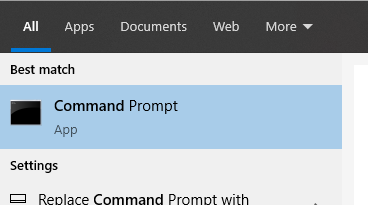
\includegraphics[width=.5\textwidth]{images/Chapter_02/CommandPrompt.png}
\end{center}

In the Command Prompt, you can do almost everything that you can do with the mouse on your computer. The command prompt starts in a specific folder on your computer, something similar to \mintinline{PowerShell}{C:\Users\User}. You can type \mintinline{bash}{dir}, and press enter to get a list of all the files and folders within that directory. If you want to navigate through your computer, you can use the command \mintinline{bash}{cd}. If you want to go one level up, you can type \mintinline{bash}{cd ..} if you want to enter into a folder, you type \mintinline{bash}{cd Folder} (where \textit{Folder} is the name of the folder you want to change to). It is out of the scope of this book to cover all the different possibilities that the Command Prompt offers, but you shouldn't have any problems finding help online. See the image below to get an idea of how things look like on Windows:

\begin{center}
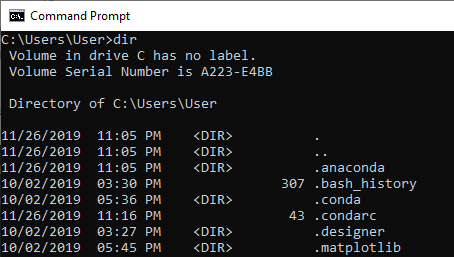
\includegraphics[width=.5\textwidth]{images/Chapter_02/CommandPrompt03.png}
\end{center}

To test that your Python installation was successful, just type \mintinline{bash}{python.exe} and hit enter. You should see a message like this:

\begin{minted}{powershell}
Python 3.7.7 (default, Oct  3 2017, 21:45:48)
[GCC 7.2.0] on Win64
Type "help", "copyright", "credits" or "license" for more information.
\end{minted}

It shows which Python version you are using and some extra information. You have just started what is called the Python Interpreter, which is an interactive way of using Python. If you come from a Matlab background, you notice its similarities immediately. Go ahead and try it with some mathematical operation like adding or dividing numbers:

\begin{minted}{pycon}
>>> 2+3
5
>>> 2/3
0.6666666666666666
\end{minted}

For future reference, when you see lines that start with \mintinline{pycon}{>>>} it means that we are working within the Python Interpreter. The lines without \mintinline{pycon}{>>>} in front are the output generated by the program.

\subsection{Adding Python to the PATH on Windows}\label{subsec:path-windows}
If you receive an error message saying that the command python.exe was not found, it means that something went slightly wrong with the installation. Remember when you selected Add Python to the PATH? That option is what tells the Command Prompt where to find the program python.exe. f, for some reason, it didn't work while installing, you have to do it manually. First, you need to find out where your Python s installed. If you paid attention during the installation process, that shouldn't be a problem. Most likely you can find it in a directory like:

\begin{minted}{powershell}
C:\Users\**YOURUSER**\AppData\Local\Programs\Python\Python36
\end{minted}

Once you find the file python.exe, copy the full path of that directory, i.e.\ the location of the folder where you found python.exe. You have to add it to the system variable called PATH:

\begin{enumerate}
 \item Open the System Control Panel. How to open it is slightly dependant on your Windows version, but it should be Start/Settings/Control Panel/System
 \item Open the Advanced tab.
 \item Click the Environment Variables button.
 \item There is a section called System Variables, select Path, then click Edit. You'll see a list of folders, each one separated from the next one by a \py{;}.
 \item Add the folder where you found the python.exe file at the end of the list (don't forget the \py{;} to separate it from the previous entry).
 \item Click OK\@.
\end{enumerate}

You have to restart the Command Prompt for it to refresh the settings. Try again to run python.exe, and it should be working now.

\subsection{Installation on Linux}\label{subsec:installation-on-linux}
Most Linux distributions come with pre-installed Python. Therefore you have to check whether it is already in your system. Open up a terminal (Ubuntu users can do Ctrl+Alt+T). You can then type \mintinline{bash}{python3}, and press enter. If it works you should see something like this appearing on the screen:

\begin{minted}{bash}
Python 3.6.3 (default, Oct  3 2017, 21:45:48)
[GCC 7.2.0] on Linux
Type "help", "copyright", "credits" or "license" for more information.
\end{minted}

If it doesn't work, you need to install Python 3 on your system. Ubuntu users can do it by running:
\begin{minted}{bash}
sudo apt install python3
\end{minted}

Each Linux distribution has a slightly different procedure to install Python, but all of them follow more or less the same ideas. After the installation, check again if it went well by typing python3 and hitting enter. Future releases of the operating system will include only Python 3 by default, and you won't need to include the \emph{3} explicitly. In case there is an error, try first running only \mintinline{bash}{python} and checking whether it recognized that you want to use Python 3.

\subsection{Installing Python Packages}\label{subsec:installing-python-packages2}\label{subsec:installing-python-packages}
One of the characteristics that make Python such a versatile language is the variety of packages that can be used in addition to the standard distribution. Python has a repository of applications called PyPI, with more than 100000 packages available. The easiest way to install and manage packages is through a command called \textbf{pip}. Pip fetches the needed packages from the repository and installs them for you. Pip is also capable of removing and upgrading packages. More importantly, Pip also handles dependencies, so you won't have to worry about them.

Pip works both with Python 3 and Python 2. To avoid mistakes, you have to be sure you are using the version of Pip that corresponds to the version of Python you want to use. If you are on Linux and you have both Python 2 and Python 3 installed, probably there are two commands, \py{pip2} and \py{3}. You should use the latter to install packages for Python 3. On Windows, you probably have to use \mintinline{PowerShell}{pip.exe} instead of just \mintinline{bash}{pip}. If, for some reason it doesn't work, you need to follow the same procedure that we explained earlier to add python.exe to the PATH, but this time with the location of your pip.exe file.

\tipsInfo{Info}{Since the moment in which Anaconda was born to nowadays, pip has gone through a very long road. Today, we can install complex packages such as numpy or PyQt directly. However, there is still some discussion regarding how much we can expect from pip at the moment of compiling programs or performing complex tasks.}

Installing a package becomes very simple. If you would like to install a package such as numpy, you should just type:
\begin{minted}{bash}
pip install numpy
\end{minted}

Windows users should instead type:
\begin{minted}{powershell}
pip.exe install numpy
\end{minted}

\warningInfo{Before Continuing}{Before installing the packages listed below, it is important to read the following section on the Virtual Environment. It helps keeping clean and separated environments for software development.}

Pip automatically grabs the latest version of the package from the repository and installs it on your computer. To follow the book, you need to install the packages listed below:
\begin{itemize}
 \item numpy -> For working with numerical arrays
 \item pint -> Allows the use of units and not just numbers
 \item pyserial -> For communicating with serial devices
 \item PyYAML -> To work with YAML files, a specially structured text file
 \item PyQt5 -> Used for building Graphical User Interfaces
 \item pyqtgraph -> Used for plotting results within the User Interfaces
\end{itemize}

\sloppy You can install all the packages with pip without trouble. If you are in doubt, you can search for packages by typing \mintinline{bash}{pip search package_name}. Usually, it is not essential the order in which you install the packages. Notice that since pip installs the dependencies as well, sometimes you get a message saying that a package is already installed even if you didn't do it manually.

To build user interfaces, we have decided to use Qt Designer, which is an external program provided by the creators of Qt. You don't need to have this program to develop a graphical application because you can do everything directly from within Python. However, this approach can be much more time consuming than dragging and dropping elements onto a window.

\subsection{Virtual Environment}\label{subsec:virtual-environment2}
When you start developing software, it is of utmost importance to have an isolated programming environment in which you can control precisely the packages installed. You can, for example, use experimental libraries without overwriting software that other programs use on your computer. With isolated environments, you can update a package only within that specific environment, without altering the dependencies in any other development you are doing.

For people working in the lab, it is even more critical to isolate different environments. In essence, you are developing a program with a specific set of libraries, each with its version and installation method. One day you, or another researcher who works with the same setup, decides to try out a program that requires slightly different versions for some of the packages. The outcome can be a disaster: If there is an incompatibility between the new libraries and the software on the computer, you could ruin the program that controls your experiment.

Unintentional upgrades of libraries can set you back several days. Sometimes it was so long since you installed a library that you can no longer remember how to do it or where to get the same version you had. Sometimes you want just to check what would happen if you upgrade a library, or you want to reproduce the set of packages installed by a different user to troubleshoot. There is no way of overestimating the benefits of isolating environments on your computer.

Fortunately, Python provides a great tool called Virtual Environment that gives you a lot of control and flexibility. A Virtual Environment is nothing more than a folder where you find copies of the Python executable and of all the packages that you install. Once you activate the virtual environment, every time you trigger pip for installing a package, it does it within that directory; the python interpreter is going to be the one inside the virtual environment and not any other. It may sound complicated, but in practice, it is incredibly simple.

You can create isolated working environments for developing software for running specific programs or for performing tests. If you need to update or downgrade a library, you are going to do it within that specific Virtual Environment, and you are not going to alter the functioning of anything else on your computer. Acknowledging the advantages of a Virtual Environment comes with time; once you lose days or even weeks reinstalling packages because something went wrong and your experiment doesn't run anymore, you will understand it.

\criticalInfo{Warning}{Virtual Environments are excellent for isolating Python packages, but many packages rely on libraries installed on the operating system itself. If you need a higher degree of isolation and reproducibility, you should check Anaconda.}

\subsubsection{Virtual Environment on Windows}
Windows doesn't have the most user-friendly command line, and some of the tools you can use for Python are slightly trickier to install than on Linux or Mac. The steps below guide you through the installation and configuration. If something is failing, try to find help or examples online. There are a lot of great examples in StackOverflow.

Virtual Environment is a python package, and therefore it can be installed with pip.

\begin{minted}{powershell}
pip.exe install virtualenv
pip.exe install virtualenvwrapper-win
\end{minted}

To create a new environment called Testing you have to run:

\begin{minted}{powershell}
mkvirtualenv Testing --python=path\to\python\python.exe
\end{minted}

The last piece is crucial because it allows you to select the exact version of Python you want to run. If you have more than one installed, you can select whether you want to use, for example, Python 2 or Python 3 for that specific project. The command also creates a folder called Testing, where it keeps all the packages and needed programs. If everything went well, you should see that your command prompt now displays a (Testing) message before the path. It means that you are indeed working inside the environment.

Once you have finished working in the environment, type:

\begin{minted}{powershell}
deactivate
\end{minted}

And you return to the normal command prompt. If you want to work on Testing again, you have to type:

\begin{minted}{powershell}
workon Testing
\end{minted}

If you want to test that things are working fine, you can upgrade pip by running:

\begin{minted}{powershell}
pip install --upgrade pip
\end{minted}

If there is a new version available, it installs it. One of the most useful commands to run within a virtual environment is:

\begin{minted}{powershell}
pip freeze
\end{minted}

It gives you a list of all the packages that you have installed within that working environment and their exact versions. So, you know what you are using, and you can revert if anything goes wrong. Moreover, for people who are worried about the reproducibility of the results, keeping track of specific packages is a great way to be sure that you can repeat everything at a later time.

You can try to install the packages listed before, such as numpy, PyQt5,  and see that they get installed only within your Test environment. If you activate/deactivate the virtual environment, the packages you installed within it are not going to be available, and you can see this with \mintinline{bash}{pip freeze}

\checkInfo{If you are using Windows Power Shell instead of the Command Prompt, there are some things that you have to change.}

\begin{minted}{powershell}
pip install virtualenvwrapper-powershell
\end{minted}

And most likely you need to change the execution policy of scripts on Windows. Open a Power Shell with administrative rights (right-click on the Power Shell icon and then select Run as Administrator). Then run the following command:

\begin{minted}{powershell}
Set-ExecutionPolicy RemoteSigned
\end{minted}

Follow the instructions that appear on the screen to allow the changes on your computer. It should allow the wrapper to work. You can repeat the same commands that we explained just before and see if you can create a virtual environment.

If it still doesn't work, don't worry too much. Sometimes there is a problem with the wrapper, but you can still create a virtual environment by running:

\begin{minted}{powershell}
virtualenv.exe Testing --python=path\to\python\python.exe
\end{minted}

Which creates the virtual environment within the Testing folder. Go to the folder Testing/Scripts and run:
\begin{minted}{powershell}
.\activate
\end{minted}

Now you are running within a Virtual Environment in the Power Shell.

\subsubsection{Virtual Environment on Linux}
On Linux, it is straightforward to install the Virtual Environment package. Depending on where you installed Python, you may need root access to follow the installation. If you are unsure, first try to run the commands without sudo, and if they fail, run them with sudo as shown below:

\begin{minted}{bash}
sudo -H pip3 install virtualenv
sudo -H pip3 install virtualenvwrapper
\end{minted}

If you are on Ubuntu, you can also install the package through apt, although we don't recommend it:
\begin{minted}{bash}
sudo apt install python3-virtualenv
\end{minted}

To create a virtual environment, you need to know where is located the version of Python that you would like to use. The easiest is to note the output of the following command:

\begin{minted}{bash}
which python3
\end{minted}

It tells you what program triggers when you run python3 on a terminal. Replace the location of Python in the following command:
\begin{minted}{bash}
mkvirtualenv Testing --python=/location/of/python3
\end{minted}

It creates a folder, usually \mintinline{bash}{~/.virtualenvs/Testing}, with a copy of the Python interpreter and all the packages that you need, including pip. That folder is the place where new modules are installed. If everything went well, you see the \mintinline{bash}{(Testing)} string at the beginning of the line in the terminal. If you see it, you know that you are working within a Virtual Environment.

To close the Virtual Environment you have to type:

\begin{minted}{bash}
deactivate
\end{minted}

To work in the virtual environment again, just do:
\begin{minted}{bash}
workon Testing
\end{minted}

If for some reason the wrapper is not working, you can create a Virtual Environment by executing:
\begin{minted}{bash}
virtualenv Testing --python=/path/to/python3
\end{minted}
And then you can activate it by executing the following command:
\begin{minted}{bash}
source Testing/bin/activate
\end{minted}

Bear in mind that in this way, you create the Virtual Environment wherever you are on your computer and not in the default folder. It can be handy if you want, for example, to share the virtual environment with somebody, or place it in a precise location on your computer.

Once you have activated the virtual environment, you can go ahead and install the packages listed before, such as numpy. You can compare what happens when you are in the working environment or outside, and check that you are isolated from the central installation. The packages that you install inside of Test are not going to be available outside of it.

One of the most useful commands to run within a virtual environment is:

\begin{minted}{bash}
pip freeze
\end{minted}

It gives you a list of all the packages that you have installed within that working environment and their exact versions. In this way, you know what you are using, and you can revert if anything goes wrong. Moreover, for people who are worried about the reproducibility of the results, keeping track of specific packages is a great way to be sure that anyone can repeat it at a later time.

\section{Qt Designer}\label{sec:install-qt-designer}
Qt Designer is a great tool to quickly build user interfaces by dragging and dropping elements to a canvas. It allows you to quickly develop elaborate windows and dialogs, styling them, and defining some basic features without writing actual code. We use this program to develop an elaborate window in which the user can tune the parameters of the experiment and display data in real-time.

If you are using \textbf{Anaconda}, the Designer comes already bundled, so you don't need to follow the steps below.

\subsection{Installing on Windows}\label{subsec:installing-on-windows}
Installing Qt Designer on Windows only takes one Python package: pyqt5-tools. Run the following command:

\begin{minted}{bash}
 pip install pyqt5-tools
\end{minted}

\sloppy And the designer should be located in a folder called \mintinline{bash}{pyqt5-tools}. The location of the folder depends on how you installed Python and whether you are using a virtual environment. If you are not sure, use the tool to find folders and files in your computer and search for \mintinline{bash}{designer.exe}.

\subsection{Installing on Linux}\label{subsec:installing-on-linux}
Linux users can install Qt Designer directly from within the terminal by running:

\begin{minted}{bash}
sudo apt install qttools5-dev-tools
\end{minted}

To start the Designer, just look for it within your installed programs, or type designer and press enter on a terminal.

The package pyqt5-tools is an independent package just aimed at making the installation of the Qt Designer easier. However, it takes a bit of time for it to update to the latest version of Python. At the time of writing, we know that it works with Python 3.7 and not with Python 3.8.

\section{Editors}\label{sec:editors}
To complete the Python For The Lab book, you need a text editor. As with many decisions in this book, you are entirely free to choose whatever you like. However, it is essential to point out some resources that can be useful to you. For editing code, you don't need anything more sophisticated than a plain text editor, such as Notepad++. It is available only for Windows, is very basic and straightforward. You can have several tabs open with different files; you can perform a search for a specific string in your opened documents or within an entire folder. Notepad++ is very good for small changes to the code, perhaps directly in the lab. The equivalent to Notepad++ on Linux is text editors such as Gedit or Kate. Every Linux distribution comes with a pre-installed text editor.

Developing software for the lab requires working with different files at the same time, being able to check that your code is correct before running it, and ideally being able to interface directly with Virtual (or Conda) Environments. For all this, there is a range of programs called IDE's or Integrated Development Environments. We strongly suggest you check \textbf{Pycharm}, which offers a free and open-source Community Edition and a Professional Edition, which you can get for free if you are a student or teacher affiliated with a University. Pycharm integrates itself with environments, allows you to install a package if it is missing, but you need it and many more things. It is a sophisticated program, but there are many great tutorials on how to get started. Familiarizing yourself with PyCharm pays off quickly.

Another very powerful IDE for Python is \textbf{Microsoft's Visual Studio}, which is very similar to Pycharm in capacities. If you have previous experience with Visual Studio, I strongly suggest you keep using it. It integrates very nicely with your workflow. Visual Studio is available not only for Windows but also for Linux and Mac. It has some excellent features for inspecting elements and help you debug your code. The community edition is free of charge. Support for Python is complete, and Microsoft has released several video-tutorials showing you how to get the best out of their program.

There are other options around, such as Atom or Sublime. However, they don't specifically target Python as the previous two. Remember that always, the choice is yours. Editors should be a tool and not an obstacle. If you have never used an IDE before, I suggest you just install PyCharm. That is what we use during the workshops, and everyone has always been very pleased with it. If you already have an IDE or a workflow with which you are happy, then keep it. If at some point, it starts failing you, you can reevaluate the situation.

\warningInfo{Tabs or Spaces}{Python is sensitive to the use of tabs and spaces. You shouldn't mix them. A standard is to use 4 spaces to indent your code. If you decide to go for a text editor, be sure to configure it such that it respects Python's stylistic choices. Notably, Notepad++ comes configured by default to use tabs instead of spaces, which is a problem if you ever copy-paste code from other sources.}
